\documentclass[../calculus.tex]{subfiles}

\begin{document}


\chapter{The Derivative}

\begin{definition}[Differentiability]
    \begin{shaded*}
        A function $f$ is differentiable at a point $x$ if the following limit exists:
        \[f'(x) = \lim_{h\to 0} \frac{f(x+h)-f(x)}{h}.\]
        For this limit to exist, both the left and right derivatives must exist and be equal.
    \end{shaded*}
\end{definition}

There are alternative, equivalent ways to express the derivative limit. For instance, letting $y = x+h$, we can write:
\[f'(x) = \lim_{y\to x} \frac{f(y)-f(x)}{y-x}.\]

Additionally, if a function is already known to be differentiable at $x$, we can evaluate the derivative using the symmetric difference quotient:
\[f'(x) = \lim_{h\to 0} \frac{f(x+h)-f(x-h)}{2h}.\]
\begin{remark}
    The existence of the symmetric limit does \textit{not} imply differentiability. For example, if $f(x) = |x|$, the symmetric limit at $x=0$ evaluates to $0$, even though the standard derivative does not exist.
\end{remark}

\begin{example}
    Let $f(x) = x^2$. We compute the derivative at $x$ using the standard limit definition:
    \begin{align*}
        f'(x) &= \lim_{h\to 0} \frac{(x+h)^2 - x^2}{h} \\
        &= \lim_{h\to 0} \frac{x^2 + 2xh + h^2 - x^2}{h} \\
        &= \lim_{h\to 0} (2x + h) = 2x.
    \end{align*}
\end{example}

Differentiability is stronger than continuity:

\begin{theorem}
    \begin{shaded*}
        If $f(x)$ is differentiable at $x=x_0$, then it is also continuous there.
    \end{shaded*}
\end{theorem}

\begin{proof}
    Suppose $f$ is differentiable at $x_0$. We want to show that $\lim_{x\to x_0} f(x) = f(x_0)$, which is equivalent to showing $\lim_{x\to x_0} (f(x) - f(x_0)) = 0$. We manipulate the limit:
    $$\lim_{x\to x_0} (f(x) - f(x_0)) = \lim_{x\to x_0} \left( \frac{f(x) - f(x_0)}{x - x_0} \cdot (x - x_0) \right).$$
    Using the algebraic properties of limits, this separates into:
    $$\lim_{x\to x_0} \frac{f(x) - f(x_0)}{x - x_0} \cdot \lim_{x\to x_0} (x - x_0) = f'(x_0) \cdot 0 = 0.$$
    Thus, $f(x) \to f(x_0)$ as $x \to x_0$, meaning $f$ is continuous at $x_0$.
\end{proof}

\begin{remark}
    The converse of this theorem is not true; a continuous function is not necessarily differentiable.
\end{remark}

\begin{example}
    Consider the function $f(x) = |x|$ at $x=0$.
    \begin{center}
    \begin{tikzpicture}[xscale=0.7, yscale=0.7]
        \draw [->] (-3, 0) -- (3, 0) node [right] {$x$};
        \draw [->] (0, -2) -- (0, 2) node [above] {$y$};
        \draw [domain=-2:0.0, samples=150, smooth] plot (\x, -\x);
        \draw [domain=0.0:2, samples=150, smooth] plot (\x, \x);
        \filldraw[red] (0,0) circle (2pt);
    \end{tikzpicture}
    \end{center}
    
    The function is continuous at $x=0$ because $\lim_{x\to 0} |x| = 0 = f(0)$. However, evaluating the left and right derivatives yields:
    \[\lim_{h\to 0^+} \frac{|0+h|-|0|}{h} = \lim_{h\to 0^+} \frac{h}{h} = 1,\]
    \[\lim_{h\to 0^-} \frac{|0+h|-|0|}{h} = \lim_{h\to 0^-} \frac{-h}{h} = -1.\]
    Since the left and right limits are not equal, the two-sided limit does not exist, and $f(x)$ is not differentiable at $x=0$.
\end{example}

Consider functions with jump discontinuities. Attempting to approximate them with smooth, polynomial functions provides useful intuition for their derivatives. If we were to connect a discontinuous jump with an approximating continuous curve, the curve would require an incredibly steep slope downwards (or upwards) at the discontinuity. As the approximation becomes exact, the connecting slope becomes vertical, meaning the right (or left) slope does not exist and tends to $\pm\infty$. A slope of $\pm\infty$ represents a vertical tangent line. This idea is illustrated below.

\begin{center}
    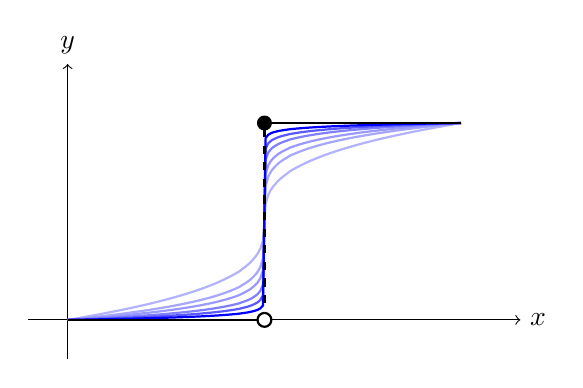
\begin{tikzpicture}[scale=2.5]
      % Axes
      \draw [->] (-0.2, 0) -- (2.3, 0) node [right] {$x$};
      \draw [->] (0, -0.2) -- (0, 1.3) node [above] {$y$};
  
      % The sequence of approximating functions
      % Increasing n makes the jump steeper. The color gets darker as n increases.
      \foreach \n in {1, 2, 3, 5, 8, 15} {
        % Calculate color intensity (capped around 100 for n=15)
        \pgfmathsetmacro\c{25 + 5 * \n};
        % Calculate the fractional exponent
        \pgfmathsetmacro\k{1 / (2*\n + 1)};
        
        % Plotting with sign and abs to safely handle negative values in fractional powers
        \draw [domain=0:2, samples=150, blue!\c!white, thick] 
          plot (\x, {0.5 + 0.5 * sign(\x - 1) * abs(\x - 1)^\k});
      }
  
      % Optional: Adding the target step function as a dashed line for visual reference
      \draw [thick, black] (0,0) -- (1,0);
      \draw [thick, black] (1,1) -- (2,1);
      \draw [dashed, thick, black] (1,0) -- (1,1);
      
      % Jump discontinuity points: open circle at (1,0), filled at (1,1)
      \draw [fill=white, thick] (1,0) circle (1pt);
      \draw [fill=black] (1,1) circle (1pt);
      
    \end{tikzpicture}
\end{center}

\begin{example}
    Suppose the position of a particle moving along a straight line at time $t$ (in seconds) is given by the function $s(t) = t^2 + 3t$ (in meters). 
    
    The average speed of the particle over the time interval $[1, 1+\Delta t]$ is the average rate of change of position:
    \[
      v_{\text{avg}} = \frac{s(1+\Delta t) - s(1)}{\Delta t} = \frac{\left((1+\Delta t)^2 + 3(1+\Delta t)\right) - (1^2 + 3(1))}{\Delta t}.
    \]
    Expanding the numerator yields:
    \[
      v_{\text{avg}} = \frac{1 + 2\Delta t + (\Delta t)^2 + 3 + 3\Delta t - 4}{\Delta t} = \frac{5\Delta t + (\Delta t)^2}{\Delta t} = 5 + \Delta t \quad (\text{for } \Delta t \neq 0).
    \]
    This tells us the average speed over any small interval starting at $t=1$. To find the \textit{instantaneous} speed of the particle at exactly $t = 1$, we take the limit as the interval length $\Delta t$ approaches $0$:
    \[
      v(1) = s'(1) = \lim_{\Delta t \to 0} (5 + \Delta t) = 5 \text{ m/s}.
    \]
\end{example}
  
\begin{example}
    Geometrically, the derivative represents the slope of the tangent line to a curve at a given point. Consider the curve defined by $f(x) = x^3 - 2x$. We wish to find the equation of the tangent line to this curve at $x = 2$.
    
    First, we find the coordinates of the point of tangency by evaluating the function: 
    \[
      f(2) = (2)^3 - 2(2) = 8 - 4 = 4.
    \]
    So, the line passes through the point $(2, 4)$. Next, we calculate the derivative $f'(x)$ to find the formula for the slope at any point $x$:
    \[
      f'(x) = \deriv{}{x}(x^3 - 2x) = 3x^2 - 2.
    \]
    Evaluating the derivative at $x = 2$ gives the slope $m$ of the tangent line:
    \[
      m = f'(2) = 3(2)^2 - 2 = 12 - 2 = 10.
    \]
    Using the point-slope form of a linear equation, $y - y_1 = m(x - x_1)$, the equation of the tangent line is:
    \[
      y - 4 = 10(x - 2) \implies y = 10x - 16.
    \]
\end{example}





\newpage

a

\end{document}